\chapter{Prototyping}
As in any product development, a few protoypes were developed.
First a smaller , 50cm wingspan aircraft with no airfoil was assembled to test and tune the flight controllers. The reduced version also enabled testing in close spaces and proximity with people with reduced danger.

With the reduced prototype proven, the larger one, photography-ready was developed. The larger one is closer to the final desired product, and is able to be used as such.

Both prototypes are described, as well as their assemblies, in the next sections.
 


\section{Reduced Scale Prototype}

A reduced prototype was used for preliminary tests of the flight controller and control systems.

Mechanically, this prototype consists of a foam board, two motors, and two control surfaces.

Smaller electronics are used as well. The servos are Turnigy 9 gram servos, The motors are AXN Floater-Jet 2208 2150KV brushless motors, the Escs are HobbyKing's RedBrick 30A ESCs, and the battery a Zippy Compact 3s 1000mah 35C.

The control surfaces were taped to the main body, and linked to the servos by a wire and plastic horn.

The motors had a custom mount 3D-Printed and fitted into the foam.

For the tests and tuning, the prototype had a hook on top, so it could be hang on the ceiling to avoid hitting the floor and walls during the tests.

The first prototype and It's components can be seen on Figure \ref{fig:smallprotorypeparts}

\begin{figure}[H]
\centering
  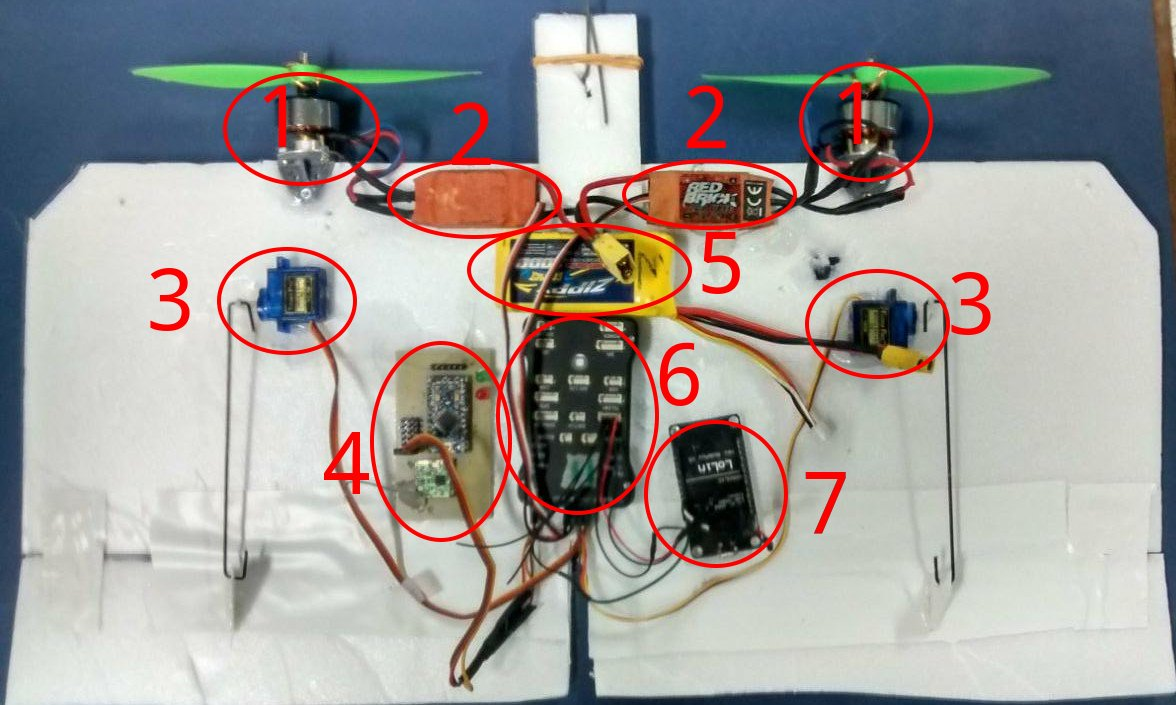
\includegraphics[width=\linewidth]{figs/reducedprototype.jpg}
  \caption{Reduced Prototype and parts:\\
   1 - Motors and 3D-printed mounts\\
   2 - HobbyKing RedBrick 30A ESCs\\
   3 - Turnigy Pro 9 gram servos\\
   4 - Diy OpenLRS 433 MHz receiver\\
   5 - Zippy Compact 3s 1000mAh 35C lithium-polymer battery\\
   6 - Pixhawk controller\\
   7 - ESP-8266 board for telemetry}
  \label{ffig:smallprotorypeparts}
\end{figure}

\section{Large Prototype}

For the larger prototype, standard RC building and fast prototyping technologies were used.
The Zag12 airfoil at root was 3D printed in 3 parts (Figure \ref{fig:printedairfoil}) then joined and insulated from the hot-wire heat with aluminum foil. For the trapezoidal wings, one side of the wire was tied to a fixed point, in such way that, if the airfoil was a circle, the wire would cut a cone on the foam. This enabled the cut of the trapezoidal wings out of foam. For the center section, two profiles were 3D-printed. their perimeters were then marked with numbers, in such way that two people, one on each side, could coordinate the hot-wire cutting process.


This process isn't perfect for the trailing edge, so some of it needs to be removed, which later gets replaced by the elevons.

The cut foam then needs to be sanded down to remove imperfections.
The half-wings are then joined with hot glue, and fiber glass spars are used to reinforce the structure.


From this point, The sections can be joined permanently or spars can be used to quickly assemble them.


With the three sections properly cut, they are glued together and sanded, and glass fiber rods were embedded and glued into the structure, two on the top and two on the bottom.

With the main structure assembled, the servos were embedded into the structure. A pocket was carved with hot wire, and two nut-holding 3D-printed parts were embedded deep into the foam and used to screw the top cover, as seem on the figure \ref{fig:servo_mount} 


\begin{figure}[H]
\centering
  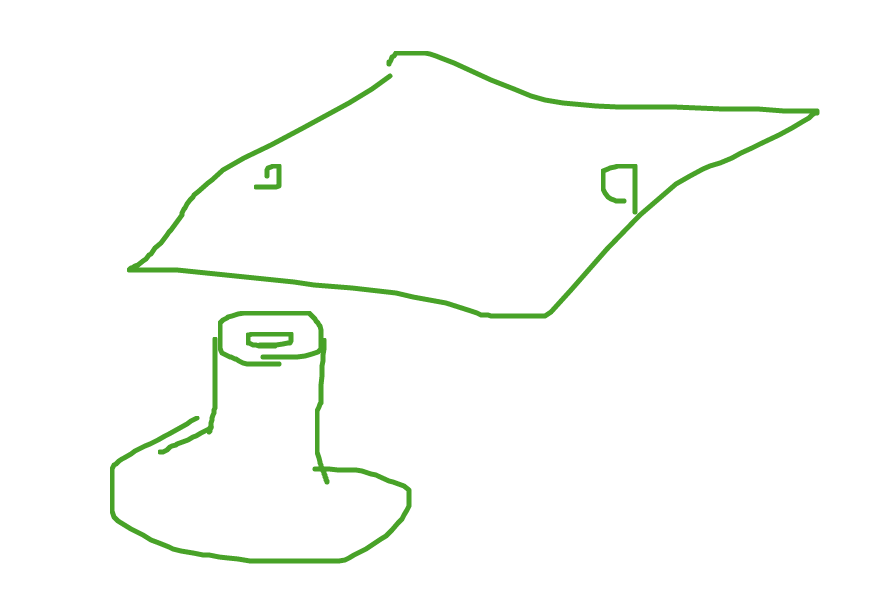
\includegraphics[width=\linewidth]{figs/servo_mount.png}
  \caption{3D-printed servo mount structure.}
  \label{fig:servomount}
\end{figure}

\begin{figure}[H]
\centering
  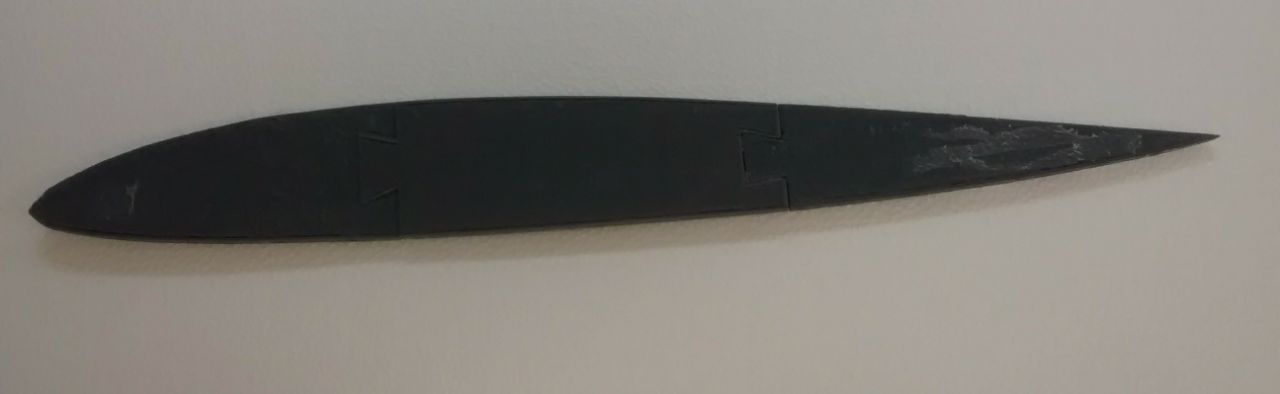
\includegraphics[width=\linewidth]{figs/printedairfoil.png}
  \caption{3D Printed Airfoil}
  \label{ffig:printedairfoil}
\end{figure}

The main structure was then covered in vinil, for aesthetial and structural purposes (the tension on the vinil helps making the structure stiffer). The vinil is a material that shrinks when heated, which makes it tension itself over it's surface.

The motor mounts were designed so they fit perfectly on the wing profile, and 3D-printed, glued, and screwed into the main wing.
The mounts can be seen on figure \ref{fig:motormount}


\begin{figure}[H]
\centering
  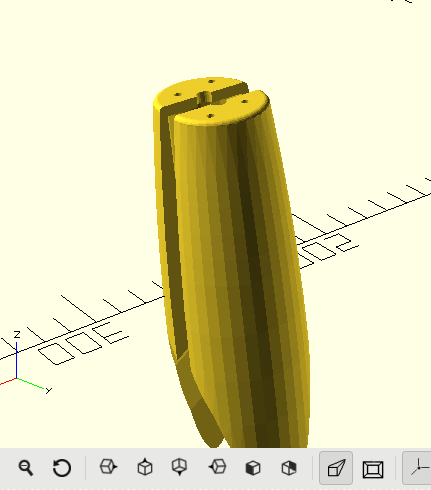
\includegraphics[width=\linewidth]{figs/motormount.png}
  \caption{3D-printed motor mount structure.}
  \label{fig:motormount}
\end{figure}


The motor mounts are also 3D-printed, and screwed into the wing.












\section{Large Prototype}